\documentclass{article}
\usepackage{amsfonts}
\usepackage{amsmath}
\usepackage{graphicx}
\usepackage{xcolor}
\usepackage{tabularx}
\usepackage{hyperref}
\hypersetup{
  colorlinks=true,
  linkcolor=blue,
  citecolor=red,
  linktoc=all,
  pdfauthor=B. Mussard,
  pdftitle=Notes on MRPT,
  pdfdisplaydoctitle=true,
  pdfpagelayout=SinglePage,
  pdfstartview=Fit,
  pdfstartpage=1,
  bookmarksopen=false
}

\newcommand  \todo[1]      {{\color{blue}[BM: #1]}}

\newcommand  \equ[2]       {\begin{align}#2\label{#1}\end{align}}
\renewcommand\b[1]         {\mathbf{#1}}
\newcommand  \var[1]       {\texttt{#1}}
\newcommand  \bra[1]       {\langle #1 \vert}
\newcommand  \ket[1]       {\vert #1  \rangle}
\newcommand  \braket[2]    {\langle  #1 \vert #2  \rangle}
\newcommand  \expect[3]    {\langle  #1 \vert #2 \vert #3 \rangle}
\newcommand  \Expect[1]    {\left\langle  #1 \right\rangle}
\newcommand  \E[2]         {\hat{E}_{#1}^{#2}}
\newcommand  \Et[2]        {\hat{\tilde{E}}_{#1}^{#2}}
\renewcommand\P            {^\prime}

\usepackage{fancyvrb}
\fvset{%
fontsize=\small,
numbers=left
}

\begin{document}

\title{Notes on MRPT}
\author{B.Mussard\\
\url{https://mussard.github.io}
}
\maketitle
\setcounter{tocdepth}{2}
\tableofcontents
\vspace*{2em}

\noindent
I'll present the equations we're solving and the setup of the codes we have.

\section{Main equations}

We want to do a perturbative addition of out-of-active-space dynamical correlation
on top of a zeroth order multi-configurational wavefunction.
The zeroth order wavefunction and energy (and the corresponding orbitals) are obtained from a CAS-like calculation.
We have the usual separation of $N_\text{c}$ core, $N_\text{a}$ active and $N_\text{v}$ virtual orbitals, and:
\equ{ }{
  \ket{\Psi_0}=\sum_n c_n\ket{D_n}
}

\subsection{Perturbation theory}

We are performing Rayleigh-Schr\"{o}dinger perturbation theory:
the partition $\hat{H}=\hat{H}_0+\hat{V}$ is so that $\ket{\Psi_0}$
and $E_0$ are eigenvector and eigenvalue of the zeroth order Hamiltonian. 
This leaves some flexibility : one can choose the Fock operator (yielding CASPT),
the Dyall Hamiltonian (yielding NEVPT) or the Fick Hamiltonian (yielding MRLCC). 
We are looking for second- and third order corrections to the energy:
\equ{eq:energies}{
  \begin{array}{rl}
  E_2&=\expect{\Psi_0}{\hat{V}}{\Psi_1}
  \\[.5em]
  E_3&=\expect{\Psi_1}{\hat{V}-E_1}{\Psi_1}
  \end{array}
}
where the first order correction to the wavefunction obeys:
\equ{eq:hylleraas}{
  (E_0-\hat{H}_0)\ket{\Psi_1}=\hat{V}\ket{\Psi_0}
}
\textit{i.e.} is found minimizing the Hylleraas functional:
\equ{}{
    \expect{\Psi_1}{E_0-\hat{H}_0}{\Psi_1}-\expect{\Psi_1}{\hat{V}}{\Psi_0}
}
In the more usual single-reference case, the inversion $\frac{1}{E_0-\hat{H}_0}$ to obtain $\ket{\Psi_1}$
is trivial, but in the multi-reference case the naive inversion in the many-particle space is problematic.
The first order wavefunction has to be computed, and this will be the subject of the following sections.

\subsection{Internal contraction}

We're going to expand Eq.(\ref{eq:hylleraas}) in a basis.
A way to expand $\ket{\Psi_1}$ (in the lhs of Eq.(\ref{eq:hylleraas})) is to use a contracted scheme,
which proposes to consider the basis of functions \textit{connected} to $\ket{\Psi_0}$.
The expansion of the first order correction to the wavefunction is then:
\equ{}{
  \ket{\Psi_1}=\sum_{I} d_I \left(\hat{E}_{I}\ket{\Psi_0}\right)
}
where $\hat{E}_{I}\ket{\Psi_0}$ are functions connected to $\ket{\Psi_0}$ through $\hat{E}_I$
and where we need to find the coefficients $\b{d}$.
The tedious part is that the basis $\{\hat{E}_{I }\ket{\Psi_0}\}$ is composed of non-orthogonal many-body states,
and the equations will involve overlaps.

\subsection{Classes}

The action of a two-electron operator on an object made of orbitals separated into
core, active and virtual orbitals
(for example in Eq.(\ref{eq:hylleraas}), $\hat{H}_0\ket{\Psi_1}$ and $\hat{V}\ket{\Psi_0}$)
can be separated into the following 8 classes of excitations in terms of the changes of the occupation pattern.

\begin{center}
\begin{tabular}{lcc|rrr|l}
  \hline\hline
  \multicolumn{3}{c|}{Names}              & $\Delta c$
                                                   & $\Delta a$
                                                        & $\Delta v$
                                                               & Operators\\
  \hline
  I    & CCVV & $V_{ij,ab }^{(0)}$  & $-2$ & $ 0$ & $+2$ & $\hat{E}_I \rightarrow \hat{E}_i^a\hat{E}_j^b$ \\
  II   & ACVV & $V_{i,ab}  ^{(-1)}$ & $-1$ & $-1$ & $+2$ & $\hat{E}_I \rightarrow \hat{E}_i^a\hat{E}_r^b$ \\
  III  & CCAV & $V_{ij,a}  ^{(+1)}$ & $-2$ & $+1$ & $+1$ & $\hat{E}_I \rightarrow \hat{E}_i^a\hat{E}_j^r$ \\
  IV   & AAVV & $V_{ab}    ^{(-2)}$ & $ 0$ & $-2$ & $+2$ & $\hat{E}_I \rightarrow \hat{E}_r^a\hat{E}_s^b$ \\
  V    & CCAA & $V_{ij}    ^{(+2)}$ & $-2$ & $+2$ & $ 0$ & $\hat{E}_I \rightarrow \hat{E}_i^r\hat{E}_j^s$ \\
  VI   & CAAV & $V_{i,a}   ^{(0)}$  & $-1$ & $ 0$ & $+1$ & $\hat{E}_I \rightarrow \hat{E}_i^a\hat{E}_s^r, \hat{E}_s^a\hat{E}_i^r$ \\
  VIII & AAAV & $V_{a}     ^{(-1)}$ & $ 0$ & $-1$ & $+1$ & $\hat{E}_I \rightarrow \hat{E}_s^r\hat{E}_r^a$ \\
  VII  & AAAC & $V_{i}     ^{(+1)}$ & $-1$ & $+1$ & $ 0$ & $\hat{E}_I \rightarrow \hat{E}_t^r\hat{E}_j^s$ \\
  \hline\hline
\end{tabular}
\end{center}
Note: the subspaces CCVV and CAAV are apart, but obviously the subspaces ACVV, CCAV,
as well as AAVV, CCAA, and AAAV, AAAC are paired two-by-two,
and the equations are very similar for each class in these pairs.

From this, the Fock space of $\ket{\Psi_1}$ is divided into the 8 subspaces,
and $\hat{H}_0$ is block-diagonal in this representation:
this allows one to solve the relevant equations in each subspace subsequently.
Everything object is expressed in sums over those classes:
\equ{}{
   & \ket{\Psi_1}=\sum_c\ket{\Psi_1^c}=\sum_c\sum_I d_I^c\left(\hat{E}_I^c\ket{\Psi_0}\right)
 \\& E_2=\sum_c E_2^c
 \\& \dots\nonumber
}

\subsection{First order correction to the wavefunction}

The coefficients $\b{d}^c$ of the expansion of the first order wavefunction in a particular class subspace,
$\ket{\Psi^c_1}$, are found with
(we use sequentially:
(a) the expression of $\ket{\Psi^c_1}$ and $\hat{V}^c\ket{\Psi_0}$ in the basis of the perturbed wavefunction,
(b) a multiplication from the left by $\bra{\Psi_0}{\hat{E}^c_K }{}^\dagger$
and (c) the realization that $(E_0-\hat{H}_0)\ket{\Psi_0}=0$):
\equ{eq:AdSw}{
 &(E_0-\hat{H}_0)\ket{\Psi^c_1}=\hat{V}^c\ket{\Psi_0}
 \\\overset{(a)}{\iff}&
 (E_0-\hat{H}_0)\sum_I  d^c_I\hat{E}^c_{I }\ket{\Psi_0}=\sum_J  w^c_J \hat{E}^c_J \ket{\Psi_0}
 \\\overset{(b)}{\iff}&
 \sum_I  \Expect{\hat{E}^c_K{ }^\dagger(E_0-\hat{H}_0)\hat{E}^c_{I }}d^c_I
=\sum_J  \Expect{ {\hat{E}^c_K }{ }^\dagger\hat{E}^c_J }w^c_J 
 \\\overset{(c)}{\iff}&
 \sum_I \Expect{ {\hat{E}^c_K }{ }^\dagger\left[(E_0-\hat{H}_0)\hat{E}^c_{I }\right]}d^c_I
=\sum_J \Expect{ {\hat{E}^c_K }{ }^\dagger\hat{E}^c_J }w^c_J 
 \\\iff&
 (\b{A}^c\b{d}^c)_K =(\b{S}^c\b{w}^c)_K 
}
to be solved for the coefficients $\b{d}^c$.
The expression of $\hat{V}^c\ket{\Psi_0}$ in the basis of $\ket{\Psi_1^c}$
can be seen as being obtained from the application of projection of the zeroth order Hamiltonian:
\equ{ }{
  \hat{V}^c\ket{\Psi_0}=\hat{P}^c\hat{H}_0\ket{\Psi_0}
  =\sum_J  \left(\hat{E}^c_J  \ket{\Psi_0}\bra{\Psi_0}{\hat{E}^c_J }{ }^\dagger\right)\hat{H}_0\ket{\Psi_0}
  =\sum_J  w^c_J  \hat{E}^c_J \ket{\Psi_0}
}
and is not always only two-electron integrals on the considered subspace
(the expression depends on the zeroth order Hamiltonian, of course!).

The terms to manipulate are $\Expect{\hat{E}_I ^c{ }^\dagger[(E_0-\hat{H}_0)\hat{E}^c_J ]}$ 
and $\Expect{\hat{E}_I ^c{ }^\dagger\hat{E}^c_J }$, 
which involve long strings of creation/annihiltion operators, 
and one can use the Wick's theorem to simplify the expressions. 
The resulting expressions will be series of tensors involving one- and two-electron integrals
(coming from $\hat{H}_0$),
and RDMs up to four order (coming from the excitation operators $\hat{E}_I$).

\todo{an example through and through}

The application of the Wick's theorem to the strings of operators is not done by hand
but with the Python library \var{sqa} and neither is the implementation of the resulting equations,
done with an interface to the C software used to calculate the energy: \var{icpt}.

\subsection{Third order correction to the energy}

The third order correction to the energy in the context of the 8 classes reads:
\equ{ }{
  E_3
  &=\expect{\Psi_1}{\hat{V}}{\Psi_1}
   =\sum_{c_1 c_2 c_{12}}
 \expect{\Psi_1^{c_1}}{\hat{V}^{c_{12}}}{\Psi_1^{c_2}}
 \nonumber\\ 
 &=\sum_{c_1 c_2 c_{12}}\sum_{I J K }
 d^{c_1}_I  w^{c_{12}}_J  d^{c_2}_K  \Expect{ \hat{E}_I ^{c_1}{}^\dagger\hat{E}_J ^{c_{12}}\hat{E}_K ^{c_2}}
 \nonumber\\ 
 &=\sum_{c_1} \sum_I  d^{c_1}_I  \sum_{c_2 c_{12}} \sum_{J K }
 w^{c_{12}}_J  d^{c_2}_K  \Expect{ \hat{E}_I ^{c_1}{}^\dagger\hat{E}_J ^{c_{12}}\hat{E}_K ^{c_2}}
 \nonumber\\ 
  &=
  \sum_{c_1} \sum_I  d^{c_1}_I  E^{c_1}_I 
}
where $c_{12}$ runs over the portions of $\hat{V}$ that
explicitly connect $\bra{\Psi_1^{c_2}}$ and $\ket{\Psi_1^{c_1}}$.

\section{Setup of codes}

\subsection{Workflow}

To obtain the second and third order correction to the energy, we need to have at hand:
\begin{enumerate}
\item a minimization engine to obtain the Hylleraas functional of Eq.(\ref{eq:hylleraas})
\item the tensor contractions involved at each step and stemming from applying the Wick's theorem to
$\Expect{\hat{E}_I ^c{ }^\dagger[(E_0-\hat{H}_0)\hat{E}^c_J ]}$ 
and $\Expect{\hat{E}_I ^c{ }^\dagger\hat{E}^c_J }$ 
\item those tensors that appear in those tensor contractions,
      \textit{i.e.} the bi-electronic integrals and the RDMS
\end{enumerate}
Figure \ref{fig:workflow} is a summary of this workflow.
\begin{figure}[!htbp]
\begin{center}
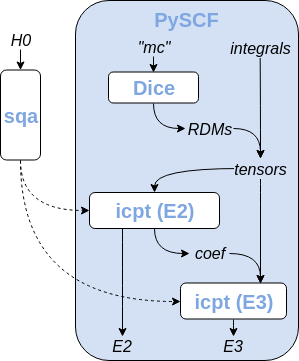
\includegraphics[width=.5\linewidth]{workflow.png}
\end{center}
\caption{Workflow}
\label{fig:workflow}
\end{figure}

\subsection{\var{PySCF} and \var{dice}}

The interface between the different cogs is implemented in \var{PySCF}.
The program is tasked with preparing all ingredients for \var{icpt} (integral tensors, RDMs tensors, input files)
and with gathering the results in one place. Hence \var{PySCF} will sequentially:
\begin{enumerate}
\item Call \var{Dice} to generate the RDMs, read the generated RDMs and write them back out in a ``npy'' format.
      It also checks that the traces are correct.
      This corresponds to lines 13-20 in the sample below.
\item Produce the integrals in MOs and write out the integral tensors in a ``npy'' format.
      This corresponds to lines 21-29 in the sample below.
\item Prepare the input files and run \var{icpt}
      for each classes and for the third order calculation.
      This corresponds to lines 30-43 in the sample below.
\end{enumerate}
The output of an MRPT run in \var{PySCF} looks like this:
\begin{Verbatim}[framesep=3mm,frame=single,framerule=2pt,rulecolor=\color{gray},numberblanklines=false]
--------------------------------------------------
                   MRPT CALCULATION
--------------------------------------------------

Perturbation type: MRLCC
With fully internally contracted scheme
With third order correction
Recognized a Density Fitting run


Number of frozen orbitals:       0
Number of core orbitals:        22
Number of active orbitals:      16
Number of virtual orbitals:     76
Number of orbitals:            114

Preparing necessary RDMs
......production of RDMs took    2015.70 sec
Reading binary 4RDM from DICE
......reading the RDM took       2687.47 sec

(GOOD) Trace 4RDM: 491400.0 =   28*   27*   26*   25
(GOOD) Trace 3RDM:  19656.0 =   28*   27*   26
(GOOD) Trace 2RDM:    756.0 =   28*   27
(GOOD) Trace 1RDM:     28.0 =   28

Producing the integrals
......production of INT took       0.22 sec

Energy_nuc  =  444.71541996
Energy_core = -3680.39510562
Energy      = -3426.93590197

WARNING: Have to use natural orbitals from CAASCF
         offdiagonal elements:    1.74383453

Basic ingredients written to /rc_scratch/bamu3429/31139/int/
......savings of INGREDIENTS took       0.89 sec

--ICPT executable:/home/bamu3429/softwares/icpt/icpt.big

Second-order:
perturber CCVV           -0.136103958              464.73
perturber CCAV           -0.017436119              227.57
perturber ACVV           -0.424424406              273.85
perturber CCAA           -0.000847298             1543.85
perturber AAVV           -0.684997895             1051.43
perturber CAAV           -0.095122227             4345.30
perturber AAAV           -0.090682806             2103.23
perturber AAAC           -0.000395028             2217.49
Total:                   -1.450009738

Third-order:              0.137398286              688.40

Total PT                 -1.312611452
Total energy          -3428.248513418
\end{Verbatim}

\subsection{\var{sqa}: Second Quantification Algebra (Python)}

The application of Wick's theorem to the expressions involved in the equations presented above
would be a cumbersome and error-prone task if done manually.
Instead, we use the \var{sqa}, that stands for ``Second Quantification Algebra'' program.
This Python library automates the manipulation of operators and in particular automates
the application of Wick's theorem.

The package lets you define categories of indexes (core, active, virtual for example)
and terms that are products of tensors and excitation operators,
and is able to enact commutation rules to the creation and destruction operators involved
to yield a Wick-ordered result.

I wrote an API to use the library, with for example one-liners that define the zeroth order Hamiltonian,
user-friendly commands to simplify the results obtained,
and systematic outputs in formats readable by \var{icpt}.
This also includes the possibility to trigger the use of the cumulant approximation for the fourth order RDM,
as well as runs adapted to the use of density-fitting for the two-electron integrals.
Hence this API basically takes as input:
\begin{itemize}
\item the zeroth order Hamiltonian (which will determine that we are doing NEVPT or MRLCC for example)
\item the class of excitations, \textit{i.e.} the excitation operators of the basis
\end{itemize}
The relevant lines of code will be found in home-made scripts in \todo{PATH}.
The output of these scripts are the ``\var{.inl}'' files containing information
on the equations that are to be handled by \var{icpt}, as shown below, where:
\begin{itemize}
\item the tensors that are going to be used are declared, lines 2-28, with
      a name, a domain in term of core, active, and virtual orbitals and a ``usage''
      (namely: amplitudes that are used in the conjugate gradient algorithm, Hamiltonian tensors,
       and density-like tensors such as RDMs and overlaps)
\item a list of tensor contractions stemming from application of the Wick's theorem, lines 29-41,
      with list of indexes, a factor, and a list of tensors involved
      (the tensors are designated by their index in the list of tensors above).
\item similar information to construct the overlap, lines 42-47
\item general information about the run to be done with \var{icpt}, lines 48-60
\end{itemize}
\begin{Verbatim}[framesep=3mm,frame=single,framerule=2pt,rulecolor=\color{gray},numberblanklines=false]
namespace MRLCC_AAVV {

  FTensorDecl TensorDecls[25] = {
    /*  0*/{"R"      , "eeaa"     , "", USAGE_Residual    },
    /*  1*/{"t"      , "eeaa"     , "", USAGE_Amplitude   },
    /*  2*/{"T"      , "eeaa"     , "", USAGE_Amplitude   },
    /*  3*/{"b"      , "eeaa"     , "", USAGE_Amplitude   },
    /*  4*/{"B"      , "eeaa"     , "", USAGE_Amplitude   },
    /*  5*/{"p"      , "eeaa"     , "", USAGE_Amplitude   },
    /*  6*/{"Ap"     , "eeaa"     , "", USAGE_Amplitude   },
    /*  7*/{"P"      , "eeaa"     , "", USAGE_Amplitude   },
    /*  8*/{"AP"     , "eeaa"     , "", USAGE_Amplitude   },
    /*  9*/{"W"      , "eeaa"     , "", USAGE_Hamiltonian },
    /* 10*/{"k"      , "aa"       , "", USAGE_Hamiltonian },
    /* 11*/{"W"      , "aaaa"     , "", USAGE_Hamiltonian },
    /* 12*/{"W"      , "aeae"     , "", USAGE_Hamiltonian },
    /* 13*/{"W"      , "aeea"     , "", USAGE_Hamiltonian },
    /* 14*/{"W"      , "caac"     , "", USAGE_Hamiltonian },
    /* 15*/{"W"      , "caca"     , "", USAGE_Hamiltonian },
    /* 16*/{"W"      , "cece"     , "", USAGE_Hamiltonian },
    /* 17*/{"W"      , "ceec"     , "", USAGE_Hamiltonian },
    /* 18*/{"k"      , "ee"       , "", USAGE_Hamiltonian },
    /* 19*/{"W"      , "e"        , "", USAGE_Intermediate},
    /* 20*/{"delta"  , "cc"       , "", USAGE_Density     },
    /* 21*/{"E2"     , "aaaa"     , "", USAGE_Density     },
    /* 22*/{"S1"     , "aaaa"     , "", USAGE_Density     },
    /* 23*/{"S2"     , "aaaa"     , "", USAGE_Density     },
    /* 24*/{"E3"     , "aaaaaa"   , "", USAGE_Density     },
  };

  FEqInfo EqsRes[11] = {
    {"abcd,ef,abeg,cdfg",       -4.0,   4, { 6,10, 5,21}},    
    {"abcd,efgh,abef,cdgh",     -2.0,   4, { 6,11, 5,21}},    
    {"abcd,efgi,abfh,cdgh,ie",   4.0,   5, { 6,14, 5,21,20}}, 
    {"abcd,efig,abfh,cdgh,ie",  -8.0,   5, { 6,15, 5,21,20}}, 
    {"abcd,eaif,bfgh,cdhg,ie",   8.0,   5, { 6,16, 5,21,20}}, 
    {"abcd,eafi,bfgh,cdhg,ie",  -4.0,   5, { 6,17, 5,21,20}}, 
    {"abcd,ae,befg,cdgf",        4.0,   4, { 6,18, 5,21}},    
    {"abcd,abef,efgh,cdgh",      2.0,   4, { 6,19, 5,21}},    
    {"abcd,efgh,abei,cdfgih",   -4.0,   4, { 6,11, 5,24}},    
    {"abcd,eafg,bghi,cdeihf",    4.0,   4, { 6,12, 5,24}},    
    {"abcd,eafg,bfhi,cdeghi",    4.0,   4, { 6,13, 5,24}},    
  };

  FEqInfo bVec[4] = {
    {"ABRS,ABPQ,RSPQ",  0.25,   3, { 3, 9,21}},
    {"BARS,ABPQ,RSQP",  0.25,   3, { 3, 9,21}},
    {"ABRS,BAPQ,RSQP",  0.25,   3, { 3, 9,21}},
    {"BARS,BAPQ,RSPQ",  0.25,   3, { 3, 9,21}},
  };

  static void GetMethodInfo(FMethodInfo &Out) {
    Out = FMethodInfo();
    Out.pName = "MRLCC_AAVV";
    Out.perturberClass = "AAVV";
    Out.Whandcoded_if_zero = 1;
    Out.E3handcoded_if_zero = 1;
    Out.pSpinClass = "restricted";
    Out.pTensorDecls = &TensorDecls[0];
    Out.nTensorDecls = 25;
    Out.EqsRes = FEqSet(&EqsRes[0], 11, "MRLCC_AAVV/Res");
    Out.bVec = FEqSet(&bVec[0], 4, "MRLCC_AAVV/bVec");
  };
};
\end{Verbatim}

\subsection{\var{icpt}: Internal Contraction PT (C)}
\label{sec:icpt}

The main command files are \var{main.cpp}, \var{icpt.cpp} and \var{PerturberDependentCode.cpp}.
The file \var{main.cpp}, commands the input file to be read and the proper job to be run
(either all NEVPT or all MRLCC jobs, or one particular job, depending on the input file).
The file \var{icpt.cpp} contains the \var{ReadInputFile} and \var{Run} routines.
The \var{Run} routine initializes everything that is needed in the \var{Init} routine
(i.e. the \var{Domains} and the \var{Tensors} as seen in the \var{.inl} file),
constructs the amplitude \var{b} in the \var{InitAmplitudes} routine,
and computes the orthogonal basis in the \var{MakeOverlapAndOrthogonalBasis} routine.
Then the conjugate gradient loop is launched, which is basically the following sequence:
\equ{}{
  P
  \xrightarrow{\text{\var{BackToNonOrthogonal}}} p
  \xrightarrow{\text{\var{ExecEquationSet}}}     Ap
  \xrightarrow{\text{\var{MakeOrthogonal}}}      AP
  \xrightarrow{\text{(loop)}}
  P^\text{new}
}
i.e. $\b{A}$ is not stored, only it's action on some tensor: $(\b{A}\b{p})$ is needed
(this is Eq.(15): $c_y=A_{xy}p_y$).

\todo{Mention Tensor, ReadNpy, where come from, TN versus TND, etc\dots}

\vspace*{1em}\hrule\clearpage
\appendix
\section{Appendices}

\subsection{Perturber space}

To help in the following, and to more closely follow derivations found in the literature, consider the zeroth order wavefunction to be an antismmetrized product of a core, an active, and a virtual part
(where all the determinant of the CAS-CI space share the same inactive part, by definition, and $\sum c_n=1$):
\equ{ }{
  \ket{\Psi_0}=\ket{D^c \Psi^a D^v}=\ket{D^c}\otimes\sum_n c_n \ket{D^a_n}\otimes\ket{D^v}=\sum_n c_n \ket{D^c D^a_n D^v}
}
Any (zeroth order) wavefunction of the Fock space outside the CAS connected to a determinant of the zeroth order wavefunction is a ``perturber wavefunctions''.
The perturber wavefunctions are of the form:
\equ{ }{
  \ket{\Psi^{c^\prime a^\prime v^\prime}_\mu}=\ket{D^{c^\prime} \Psi^{a^\prime}_\mu D^{v^\prime}}=\sum_I c^{c^\prime a^\prime v^\prime}_{\mu,I} \ket{D^{c^\prime} D^{a^\prime}_I D^{v^\prime}}
}
where the occupation pattern is changed, with respect to the CAS-CI space, by $c^\prime$, $v^\prime$ and $a^\prime$ electrons in the core, virtual and active spaces
(all three changes can be zero, negative or positive, see below)
and where $\mu$ labels the different perturbers.
Note that in the literature $a^\prime$ is called $k$ and $l$ is used to collectively designates $(c^\prime v^\prime)$.

Now that this is established, we can simplify the notations back to a more condensed form.
The determinants seen in the previous equation can be written as excitations to determinants of the zeroth order wavefunction:
\equ{ }{
  \ket{D^{c^\prime} D^{a^\prime}_I D^{v^\prime}}
  =\ket{\hat{E}^{c^\prime}\!\!    D^{c}  \;\;
        \hat{E}^{a^\prime}_{I,n}  D^{a}_n\;\;
        \hat{E}^{v^\prime}\!\!    D^{v}}
  =\hat{E}^{c^\prime a^\prime v^\prime}_{I,n}\ket{D^c D^a_n D^v}
  =\hat{E}^c_{I,n}\ket{D_n}
}
where $(c)$ collectively designate the ``class of excitation'' $(c^\prime a^\prime v^\prime)$
(see below). 
The perturber wavefuntions belong to the total Fock space $S=\bigoplus S^c$, where $S^c$ are the Fock spaces spanned by the basis:
\equ{ }{
  b=\{\hat{E}^c_{I,n}\ket{D_n}\}
}
and all the objects interesting in this context are decomposed as follow:
\equ{ }{
  \hat{E}_{I,n}=\sum \hat{E}_{I,n}^c
  \text{,}\qquad
  \ket{\Psi_1}=\sum \ket{\Psi_1^c}
  \text{,}\qquad
  \hat{V}=\sum \hat{V}^c
  \text{,}\qquad
  E_2=\sum E_2^c
  \text{, etc\dots}
}

\paragraph{Uncontracted scheme}

The uncontracted scheme exploits the full dimentionnality of the Fock space of the perturber wavefunctions, that is to say it proposes to expand the perturber wavefunction $\ket{\Psi^c_\mu}$ in the basis:
\equ{ }{
  b_\text{UC}=b=\{\hat{E}^c_{I,n}\ket{D_n}\}
  \qquad\text{and}\qquad
  \ket{\Psi^c_\mu}=\sum_I c^c_{\mu,I} \hat{E}^c_{I,n}\ket{D_n}
}
The perturber wavefunctions could be defined as the eigenfunctions of the Hamiltonian in the spaces $S^c$,
that is to say that the $c^c_{\mu,I}$ coefficients could be obtained by diagonalization of the Hamiltonian in $S^c$, which is a very expensive calculation.
The first order correction to the wavefunction would then be expanded on the perturber wavefunctions:
\equ{ }{
  \ket{\Psi_1}=\sum_{c} \ket{\Psi_1^c}
  \qquad\text{and}\qquad
  \ket{\Psi_1^c}=\sum_{c \mu} c^c_\mu \ket{\Psi^c_\mu}
}
but we are actually only interested in the coefficients $d^c_{I,n}$ of the expansion of $\ket{\Psi_1}$ directly on the basis $b_\text{UC}$:
\equ{ }{
  \ket{\Psi_1}=\sum_{c} \ket{\Psi_1^c}
  \qquad\text{and}\qquad
  \ket{\Psi_1^c}=\sum_{c I} d^c_{I,n} \hat{E}^c_{I,n}\ket{D_n}
}
that can be found using equations like those found later in these notes (see HERE). This is a less expensive calculation, although a large number of linear equation of excited CAS-CI size have to be perfomed\dots

\paragraph{Internal contraction}
\label{sec:contraction}

An alternative way would be to use a contracted scheme, which rather proposes to consider subspaces $\bar{S}^c\supset S^c$ of perturber wavefunctions connected to $\ket{\Psi_0}$ (by opposition to perturber wavefunctions connected to a determinant of $\ket{\Psi_0}$). The basis of such subspaces are:
\equ{ }{
  b_\text{IC}=\{\hat{E}_{I}^c\ket{\Psi_0}\}
}
and the expansion of the first order correction to the wavefunction becomes:
\equ{}{
  \ket{\Psi_1}=\sum_{c}\ket{\Psi_1^c}\qquad\text{and}\qquad \ket{\Psi_1^c}=\sum_{I } d^c_I \hat{E}^c_{I}\ket{\Psi_0}=\sum_{I } d^c_I \hat{E}^c_{I}\sum_n c_n\ket{D_n}}
The contraction is a factorization, much like CC is a factorization of the parameters of FCI, and you can get (approximations to) the original coefficients $d^c_{I,n} $ by products of $c_n$ and $d^c_I$ coefficients.

There is different level of contraction depending of the definition chosen for the excitation operators $\hat{E}_I^c$. A strongly contracted scheme would consider only one perturber wavefunction per class of excitation, found by application of the perturbation operator (i.e. by a part of the Hamiltonian):
\equ{}{
  \bar{S}^c=\text{span}(\hat{V}^c\ket{\Psi_0})
  \qquad\text{and}\qquad
  \hat{E}^c_I =\hat{V}^c = \hat{P}^c \hat{H}
}
The coefficients $d^c_I$ are determined by formulas.
The tedious part is that the basis $\{\hat{E}_{I }\ket{\Psi_0}\}$ is composed of non-orthogonal many-body states, and the equations will involve overlaps (see Subsection \ref{sec:derivOverlaps} \nameref{sec:derivOverlaps} and \ref{sec:overlaps} \nameref{sec:overlaps}).

\subsection{Perturbation tensor}
\label{sec:Wtensor}

For some classes of excitations (namely CAAV, AAAV and AAAC), we do not have merely $w^c_J =W^c_J $ ($W$ being the tensor of corresponding integrals).
In the program (see Section \ref{sec:icpt}: \nameref{sec:icpt}), this is handled by adding the desired terms to the $W$ that is to be contracted with the overlap.
%(See Section IV.F of AngCimMal-JCP-2002)
%(See Section IV.G of AngCimMal-JCP-2002)
%(See Section IV.H of AngCimMal-JCP-2002)

\paragraph{CAAV}
\equ{ }{
  (ri,\mu)&=\sum_{\substack{ab\\ a\P b\P}} 2W1_{ab}^{ri}\Expect{\E{a\P}{b\P}\E{b}{a}} c_{a\P b\P}^\mu
           -\sum_{\substack{ab\\ a\P b\P}}  W2_{ab}^{ri}\Expect{\E{a\P}{b\P}\E{b}{a}} c_{a\P b\P}^\mu
          \nonumber\\&
           +\sum_{ab}                      2h^{ri}      \Expect{\E{a\P}{b\P}}         c_{a\P b\P}^\mu
          \nonumber\\&
           =\sum_{\substack{ab\\ a\P b\P}} 2W1_{ab}^{ri}\Expect{\E{a\P}{b\P}\E{b}{a}} c_{a\P b\P}^\mu
           -\sum_{\substack{ab\\ a\P b\P}}  W2_{ab}^{ri}\Expect{\E{a\P}{b\P}\E{b}{a}} c_{a\P b\P}^\mu
          \nonumber\\&
           +\sum_{\substack{ab\\ a\P b\P}} 2h^{ri}\frac{\delta_{a\P b\P}}{N_\text{a}}
                                                        \Expect{\E{a\P}{b\P}\E{b}{a}} c_{a\P b\P}^\mu
\nonumber\\                                                        
  (ri,\mu)\P
         &=-\sum_{\substack{ab\\ a\P b\P}}  W1_{ab}^{ri}\Expect{\E{a\P}{b\P}\E{b}{a}} c_{a\P b\P}^\mu
           +\sum_{\substack{ab\\ a\P b\P}}  W2_{ab}^{ri} S^{\prime\prime}_{a\P b\P,ab}c_{a\P b\P}^\mu
          \nonumber\\&
           -\sum_{ab}                       h^{ri}      \Expect{\E{a\P}{b\P}}         c_{a\P b\P}^\mu
          \nonumber\\&
          =-\sum_{\substack{ab\\ a\P b\P}}  W1_{ab}^{ri}\Expect{\E{a\P}{b\P}\E{b}{a}} c_{a\P b\P}^\mu
           +\sum_{\substack{ab\\ a\P b\P}}  W2_{ab}^{ri} S^{\prime\prime}_{a\P b\P,ab}c_{a\P b\P}^\mu
          \nonumber\\&
           -\sum_{\substack{ab\\ a\P b\P}}  h^{ri}\frac{\delta_{a\P b\P}}{N_\text{a}}
                                                        \Expect{\E{a\P}{b\P}\E{b}{a}} c_{a\P b\P}^\mu
}
\equ{ }{
  W1_{ab}^{ri}\leftarrow W1_{ab}^{ri}+h^{ri} \frac{\delta_{a\P b\P}}{N_\text{a}}
}

\paragraph{AAAV}

\equ{ }{
  (r,\mu)&=\sum_{\substack{abc\\ a\P b\P c\P}} W^r_{abc}\Expect{\E{a\P}{c\P}\E{b}{b\P}\E{c}{a}}c_{a\P b\P c\P}^\mu
          +\sum_{\substack{abc\\ a\P b\P c\P}} {h\P}_b^r\Expect{\E{a\P}{c\P}\E{b}{b\P}}        c_{a\P b\P c\P}^\mu
          \nonumber\\&
          =\sum_{\substack{abc\\ a\P b\P c\P}} W^r_{abc}\Expect{\E{a\P}{c\P}\E{b}{b\P}\E{c}{a}}c_{a\P b\P c\P}^\mu
          +\sum_{\substack{abc\\ a\P b\P c\P}} {h\P}_b^r \frac{\delta_{ca}}{N_\text{a}}
                                                        \Expect{\E{a\P}{c\P}\E{b}{b\P}\E{c}{a}}c_{a\P b\P c\P}^\mu
}
\equ{ }{
  W_{abc}^{r}\leftarrow W_{abc}^{r}+{h\P}_b^r \frac{\delta_{ca}}{N_\text{a}}
}

\paragraph{AAAC}

\equ{ }{
  (i,\mu)&=\sum_{\substack{abc\\ a\P b\P c\P}} W^i_{cba}\Expect{\E{a\P}{c\P}\Et{b}{b\P}\E{c}{a}}c_{a\P b\P c\P}^\mu
          +\sum_{\substack{abc\\ a\P b\P c\P}} {h\P}_b^i\Expect{\E{a\P}{c\P}\Et{b}{b\P}}        c_{a\P b\P c\P}^\mu
          \nonumber\\&
          =\sum_{\substack{abc\\ a\P b\P c\P}} W^i_{cba}\Expect{\E{a\P}{c\P}\Et{b}{b\P}\E{c}{a}}c_{a\P b\P c\P}^\mu
          +\sum_{\substack{abc\\ a\P b\P c\P}} {h\P}_b^i \frac{\delta_{ca}}{N_\text{a}}
                                                        \Expect{\E{a\P}{c\P}\Et{b}{b\P}\E{c}{a}}c_{a\P b\P c\P}^\mu
}
\equ{ }{
  W_{abc}^{i}\leftarrow W_{abc}^{i}+{h\P}_b^i \frac{\delta_{ca}}{N_\text{a}}
}

\subsection{Sketch derivation of the overlaps}
\label{sec:derivOverlaps}

A sketch derivation of the overlaps involved in the different classes might help, notably in realizing that the overlap only contains active space indexes.

\paragraph{ACVV}
\equ{ }{
  \Expect{ \E{a\P}{p\P}\E{b\P}{i\P}\E{i}{b}\E{p}{a}}
}
where, going from the center, one cannot destroy a $b\P$ that has not been created, so this gives rise to a $\delta_{b\P b}$ or $\delta_{b\P a}$ (and later a $\delta_{a\P b}$ or $\delta_{a\P a}$).
Then one cannot create a $i\P$ that has not been destroyed, so this gives rise to a $\delta_{i\P i}$. 
One is left with a $\Expect{\E{p}{p\P}}=E_1(aa)$.

\paragraph{CCAV}
\equ{ }{
  \Expect{ \E{p\P}{i\P}\E{a\P}{j\P}\E{j}{a}\E{i}{p}}
}
where, going from the center, one cannot destroy a $a\P$ that has not been created, so this gives rise to a $\delta_{a\P a}$.
Then one cannot create a $j\P$ that has not been destroyed, so this gives rise to a $\delta_{j\P j}$ or $\delta_{j\P i}$ (and later to a $\delta_{i\P j}$ or $\delta_{i\P i}$).
One is left with a $\Expect{\E{p\P}{p}}=\tilde{E}_1(aa)$.

\paragraph{AAVV}
\equ{ }{
  \Expect{ \E{a\P}{p\P}\E{b\P}{q\P}\E{q}{b}\E{p}{a}}
}
where, going from the center, one cannot destroy a $b\P$ that has not been created, so this gives rise to a $\delta_{b\P b}$ or $\delta_{b\P a}$ (and later to a $\delta_{a\P b}$ or $\delta_{a\P a}$).
One is left with a $\Expect{\E{p}{p\P}\E{q}{q\P}}=E_2(aaaa)$.

\paragraph{CCAA}
\equ{ }{
  \Expect{ \E{p\P}{i\P}\E{q\P}{j\P}\E{j}{q}\E{i}{p}}
}
where, going from the center, one cannot create a $j\P$ that has not been destroyed, so this gives rise to a $\delta_{j\P j}$ or $\delta_{j\P i}$ (and later to a $\delta_{i\P j}$ or $\delta_{i\P i}$).
One is left with a $\Expect{\E{p\P}{p}\E{q\P}{q}}=\tilde{E}_2(aaaa)$.

\paragraph{CAAV}
\equ{ }{
  \Expect{ \E{p\P}{i\P}\E{a\P}{q\P}\E{q}{a}\E{i}{p} }
  ,\quad
  \Expect{ \E{p\P}{q\P}\E{a\P}{i\P}\E{i}{a}\E{q}{p} }
  ,\quad
  \Expect{ \E{p\P}{q\P}\E{a\P}{i\P}\E{q}{a}\E{i}{p} }
}
which will give rise to $\delta_{i\P i}$ and $\delta_{a\P a}$, and an overlap that only depend on $pq,p\P q\P$ in different order that give rise to $E_2$ and $E_1$.)

\paragraph{CCVV}
\equ{ }{
  \Expect{ \E{a\P}{i\P}\E{b\P}{j\P}\E{j}{b}\E{i}{a}}
}
where, going from the center, one cannot destroy a $b\P$ that has not been created, so this gives rise to a $\delta_{b\P b}$ or $\delta_{b\P a}$.
Similarly, one cannot create a $j\P$ that has not been destroyed, so this gives rise to a $\delta_{j\P j}$ or $\delta_{j\P i}$.
Then a $\delta_{a\P b}$ or $\delta_{a\P a}$ and a $\delta_{i\P j}$ or $\delta_{i\P i}$.


\subsection{More on the overlaps}
\label{sec:overlaps}

In the code, the overlaps are computed and then diagonalized to solve Eq.~\ref{eq:AdSw} in an orthogonal basis. This is how it's thought.
The overlap is diagonalized as follow:
\equ{}{&
  \b{S}\b{U}=\b{U}\b{D}
     \\&
  \b{U}^\dagger\b{S}\b{U}=\b{U}\b{S}\b{U}^\dagger=\b{D}
     \\&
  \b{U}^\dagger\b{U}=\b{U}\b{U}^\dagger=\b{1}
}
and the orthogonal basis transformation is defined:
\equ{}{&
  \b{V}=\b{U}\b{D}^{-1/2}
     \\&
  \b{V}\b{D}\b{V}^\dagger=\b{D}\b{V}^\dagger \b{V}=\b{V}^\dagger \b{V}\b{D}=\b{1}
     \\&
  \b{V}^\dagger\b{S}\b{V}=\b{1}
}
so that the equation to solve becomes:
\equ{}{&
  \b{A}\b{d}=\b{S}\b{w}
     \\&
  \b{V}^\dagger \b{A} (\b{V}\b{D}\b{V}^\dagger) \b{d} = \b{V}^\dagger \b{S} (\b{V}\b{D}\b{V}^\dagger) \b{w}
     \\&
  \tilde{\b{A}} \tilde{\b{d}} = \tilde{\b{w}}
}
where:
\equ{}{&
  \tilde{\b{A}}=\b{V}^\dagger \b{A} \b{V}
     \\&
  \tilde{\b{d}}=\b{D}\b{V}^\dagger \b{d}=\b{D}^{1/2}\b{U}^\dagger \b{d}
     \\&
  \tilde{\b{w}}=\b{D}\b{V}^\dagger \b{w}=\b{D}^{1/2}\b{U}^\dagger \b{w}
}

\paragraph{ACVV}

We are considering $(i,p)\rightarrow(a,b)$, but it is important to distinguish between $t_{ip}^{ab}$ and $t_{pi}^{ab}$. By restricting to $a< b$, we obtain:
\equ{ }{
  \b{S}_1=\begin{pmatrix} 2 E_1 & -E_1 \\ -E_1 & 2 E_1 \end{pmatrix}
}
and when $a=b$, $\b{S}_2=E_1$. 
Historically, in the code, this explained the presence of two tensors: \var{S1:AA} and \var{S2:aa}, where \var{A} stands for a domain twice as big as \var{a}, allowing a block structure.
We had:
\equ{ }{
  \begin{pmatrix}T_{ip}^{ab}\\T_{pi}^{ab}\end{pmatrix}
  =
  \begin{pmatrix}
    (V_a)_{p p\P} & (V_b)_{p p\P}\\
    (V_c)_{p p\P} & (V_d)_{p p\P}
  \end{pmatrix}
  \begin{pmatrix}t_{ip\P}^{ab}\\t_{p\P i}^{ab}\end{pmatrix}
  =
  \begin{pmatrix}
    V_a t_{ip\P}^{ab} + V_b t_{p\P i}^{ab} \\
    V_c t_{ip\P}^{ab} + V_d t_{p\P i}^{ab}
  \end{pmatrix}
}
and in the case where $a=b$, $T=\b{V}_2 t$. The matrices $V_a$, $V_b$, $V_c$ and $V_d$ were blocks of the orthogonal basis $\b{V}_1$ formed from the block matrix $\b{S}_1$.
Now we use the fact that given the block structure of $\b{S}_1$, its eigenvectors and eigenvalues are: 
\equ{ }{
  \b{U}=
}
where\dots

\paragraph{CCAV}

This case is exactly similar to the previous one, with $(i,j)\rightarrow(p,a)$ and the restriction $i<j$. The 1RDM $E_1$ is replaced with the one-hole RDM $\tilde{E_1}=2\text{I} - E_1$, so that we had in the code:
\equ{ }{
  \b{S}_1=\begin{pmatrix} 2\tilde{E_1} & -\tilde{E_1}\\ -\tilde{E_1} & 2\tilde{E_1} \end{pmatrix}
         =\begin{pmatrix}-2 E_1   &   E_1    \\  E_1     & -2 E_1  \end{pmatrix}
         +\begin{pmatrix} 4\text{I} & -2\text{I} \\ -2\text{I} & 4\text{I} \end{pmatrix}
}
and $\b{S}_2=\tilde{E_1}=2\text{I}-E_1$.
We know use the same reasonning as for ACVV to handle only \var{aa}-size matrices.

\paragraph{AAVV}

We are considering $(p,q)\rightarrow(a,b)$, with $a<b$. Restricting ourselves to $p<q$, we have:
\equ{ }{
  \b{S}_1=\begin{pmatrix} E_2 & E_2^\dagger \\ E_2^\dagger & E_2 \end{pmatrix}
}
and for $a=b$, $\b{S}_2=E_2+E_2^\dagger$.
Historically, this explained the dimension of $\b{S}_1$ being \var{S1:aAaA} 
We had:
\equ{}{
  \begin{pmatrix}T_{pq}^{ab}\\T_{qp}^{ab}\end{pmatrix}
  =
  \begin{pmatrix}
    (V_a)_{pq,p^\prime q^\prime}  & (V_b)_{pq,p^\prime q^\prime} \\
    (V_c)_{pq,p^\prime q^\prime}  & (V_d)_{pq,p^\prime q^\prime} \\
  \end{pmatrix}
  \begin{pmatrix}t_{p^\prime q^\prime}^{ab}\\t_{q^\prime p^\prime}^{ab}\end{pmatrix}
}
where the matrices $V_a$, $V_b$, $V_c$ and $V_d$ were blocks of the orthogonal basis $\b{V}_1$ formed from the block matrix $\b{S}_1$.
Now we use the fact that given the block structure of $\b{S}_1$, its eigenvectors and eigenvalues are: 
\equ{ }{
  \b{U}=\begin{pmatrix}
         -\b{u} & \b{u} \\
          \b{u} & \b{u} \\
        \end{pmatrix}
  \b{D}=\begin{pmatrix}
    \b{d}-\b{dt} & \b{0} \\
    \b{0} & \b{d}-\b{dt} \\
        \end{pmatrix}
}

\paragraph{CCAA}

This case is exactly similar to the previous one, with $(i,j)\rightarrow(p,q)$. The 2RDM $E_2$ is replaced with the twohole RDM $\tilde{E_2}=E_2+\delta E_1-2\delta E_1 -2\delta\delta +4\delta\delta$. That is why the overlaps are a little bit more fastidious to accumulate and historically we resorted to \var{MakeS1} and \var{MakeS2}. In the code we do not use a doubled dimension \var{A=2*a}.

\paragraph{CAAV}

Similarly, we have to distinguish between $t_{ip}^{qa}$ and $t_{pi}^{qa}$, which are spanned by two different basis. We have:
\equ{ }{
  \b{S}=\begin{pmatrix}
    A & B \\ B & C
  \end{pmatrix}
}
where
\equ{ }{
  A_{pq,p\P q\P}&=2{E_2}_{pq,p\P q\P} +2\delta_{p p\P} {E_1}_{q q\P}\\
  B_{pq,p\P q\P}&=-{E_2}_{pq,p\P q\P} - \delta_{p p\P} {E_1}_{q q\P}\\
  C_{pq,p\P q\P}&=-{E_2}_{pq,q\P p\P} +2\delta_{p p\P} {E_1}_{q q\P}
}

\noindent
\underline{Note:} in the program, the $(4 N_\text{a}^4)$ are distributed as $2N_\text{a}^2.2N_\text{a}^2$, i.e. as $S_1(pQ,rS)$, i.e. as a two-dimensionnal array.

\noindent
\underline{Note:} in the program, for AAVV, we had the $(4 N_\text{a}^4)$ distributed as $N_\text{a}.2N_\text{a}.N_\text{a}.2N_\text{a}$, i.e. as $S_1(p,Q,r,S)$, i.e. for each $p,r$, we have:

\equ{ }{
  \begin{pmatrix}
    qs & qs \\ qs & qs
  \end{pmatrix}
}

\paragraph{CCVV}

\todo{I though the overlap of this class is made of $\delta$ functions, there is $1/\sqrt{2}$ and $1/\sqrt{3}$ that arise : I should check that (norm?).}

The $(ij)\rightarrow(ab)$ are separated in four components (with $i<j$ and $a<b$): $t_1\equiv t_{ij}^{ab}$, $t_2\equiv t_{ji}^{ab}$, $t_3\equiv t_{ij}^{ba}$, $t_4\equiv t_{ji}^{ba}$. We have:
\equ{}{
  \begin{pmatrix}T_1\\T_2\\T_3\\T_4\end{pmatrix}
  =
  \frac{1}{4}
  \begin{pmatrix}
    1 & 1 & 1 & 1\\
    1\sqrt{3} & -1\sqrt{3} & -1\sqrt{3} & 1\sqrt{3} \\
    & -- & -- & \\
    & -- & -- & 
  \end{pmatrix}
  \begin{pmatrix}t_1\\t_2\\t_3\\t_4\end{pmatrix}
}
and in the case where $a=b$, we end up with:
\equ{}{
  \begin{pmatrix}T_1\\T_2\end{pmatrix}
  =
  \frac{1}{2}
  \begin{pmatrix}
    1\sqrt{2} & 1\sqrt{2}\\
    -- & -- \\
  \end{pmatrix}
  \begin{pmatrix}t_1\\t_2\end{pmatrix}
}
The reverse transformation reads: 
\equ{}{
  \frac{1}{4}
  \begin{pmatrix}t_1\\t_2\\t_3\\t_4\end{pmatrix}
  =
  \begin{pmatrix}
    1 & \sqrt{3} & \\
    1 &-\sqrt{3} & -- & -- \\
    1 &-\sqrt{3} & -- & -- \\
    1 & \sqrt{3} & 
  \end{pmatrix}
  \begin{pmatrix}T_1\\T_2\\T_3\\T_4\end{pmatrix}
  \\\text{and:}\qquad\quad
  \begin{pmatrix}t_1\\t_2\end{pmatrix}
  =
  \frac{1}{2}
  \begin{pmatrix}
    1\sqrt{2} & --\\
    1\sqrt{2} & --\\
  \end{pmatrix}
  \begin{pmatrix}T_1\\T_2\end{pmatrix}
}


\paragraph{About $E.W$}

With $E2^\dagger_{pq,rs}=E2_{pq,sr}$ and $W^{ab}_{rs}=<ab|rs>=W1^{ab}_{rs}$ and $W^{ba}_{rs}=<ba|rs>=W2^{ab}_{sr}$, we have:
\equ{ }{
  (E2.W1)^{ab}_{pq}
  & =\sum_{rs} E2_{pq,rs} W1^{ab}_{rs}
 \nonumber\\
 & =\sum_{sr} E2_{pq,sr} W1^{ab}_{sr}
 \nonumber\\
 & =\sum_{rs} E2^\dagger_{pq,rs} W2^{ab}_{rs}
 \nonumber\\
 & =(E2^\dagger.W2)^{ab}_{pq}
}
\equ{ }{
  (E2^\dagger.W1)^{ab}_{pq}
  & =\sum_{rs} E2^\dagger_{pq,rs} W1^{ab}_{rs}
 \nonumber\\
 & =\sum_{rs} E2_{pq,sr} W1^{ab}_{rs}
 \nonumber\\
 & =\sum_{sr} E2_{pq,rs} W2^{ab}_{rs}
 \nonumber\\
 & =(E2.W2)^{ab}_{pq}
}

\subsection{More details about \var{sqa}}

The useful object the library has are:

\noindent
\begin{tabularx}{\linewidth}{lX}
  \var{sqa.index}      & associates a kind to an index (core, active, virtual).
                         These indexes can be make to be dummy indexes or not.\\
  \var{sqa.sfExOp}     & defines a ``spin free excitation operator'' $\E{m\dots}{n\dots}$ \\
  \var{sqa.symmetry}   & defines a ``symmetry class'' applicable to any tensor  \\
  \var{sqa.tensor}     & defines a ``tensor'', with a name, indexes and \var{sqa.symmetry} classes: $t^{m\dots}_{n\dots}$  \\
  \var{sqa.term}       & defines a ``term'' of an equation with \var{sqa.tensor} and \var{sqa.sfExOp} \\
  \var{sqa.commutator} & defines a ``commutator'' of two \var{sqa.term}s  \\
\end{tabularx}

\vspace{.5cm}
\noindent
The actions on these objects that are interesting for us are:

\noindent
\begin{tabularx}{\linewidth}{lX}
  \var{sqa.multiplyTerms}               & creates an \var{sqa.term} that is the multiplication of two \var{sqa.term}s\\
  \var{sqa.normalOrder}                 & normal orders a string of \var{sqa.term}s \\
\end{tabularx}

%and the simplification of results are done with
%
%\begin{tabularx}{\linewidth}{lX}
%  \var{sqa.contractCoreOps}             & set \var{sqa.term}s that contain only core indexes to delta-functions \\
%  \var{sqa.removeVirtOps}               & set \var{sqa.term}s that contain only virtual indexes to 0  \\
%  \var{sqa.termChop}                    & simplifies a string of \var{sqa.term}s (1/2)  \\
%  \var{sqa.combineTerms}                & simplifies a string of \var{sqa.term}s (2/2)  \\
%  \var{contractDeltaFuncs\_new}         & (handling of indexes and delta-functions)\\
%  \var{replaceRepeatIndicesWithDeltas}  & (handling of indexes and delta-functions)\\
%  \var{replaceSingleKdeltaWithDeltas}   & (handling of indexes and delta-functions)\\
%  \var{replaceAllKdeltaWithDeltas}      & (handling of indexes and delta-functions)\\
%\end{tabularx}

\vspace{.5cm}
\noindent
We want to handle expressions like (in the example of CCVV, with $\hat{E}^\dagger_I =\E{d}{l}\E{c}{k}$ and $\hat{E}_J =\E{j}{b}\E{i}{a}$):
\equ{ }{
  A_{I J }=\Expect{\E{d}{l}\E{c}{k}[\hat{H}_0\E{j}{b}\E{i}{a}]}
  \qquad\text{ and }\qquad
  S_{I J }=\Expect{\E{d}{l}\E{c}{k}\E{j}{b}\E{i}{a}}
}
Defining the zeroth order Hamiltonian is a simple matter of calling for example:
\begin{verbatim}
H=h0('MRLCC',df=True)
\end{verbatim}
Then, one will want to associate indexes as such:
\begin{verbatim}
list = gimme('vvcc')
\end{verbatim}
Then one actually wants to obtain equations for $(Ap)_I  = A_{I J }.p_J $, so that one will writethe following piece of code:
\begin{verbatim}
Cin  = sqa.tensor("p",  [a,b,i,j], [Dsym_c])
Cout = sqa.tensor("Ap", [c,d,l,k], [Dsym_c])
Op1 = sqa.term( 1.0, [""],  [Cin,  sqa.sfExOp([a, i]) , sqa.sfExOp([b, j])])
Op2 = sqa.term( 1.0, [""],  [Cout, sqa.sfExOp([k, d]) , sqa.sfExOp([l, c])])
commutator = []
commutator +=  sqa.commutator(HD_A, Op1)
commutator +=  sqa.commutator(T_C,  Op1)
commutator +=  sqa.commutator(T_A,  Op1)
commutator +=  sqa.commutator(T_V,  Op1)
\end{verbatim}
where \var{Cin="p"} is a container for the current trial vector, and \var{Cout="Ap"} is a container for the updated trial vector.
\begin{verbatim}
result = []
for t in commutator:
    result += sqa.normalOrder(sqa.multiplyTerms(Op2, t))
result = simplify_all(result,[deltaC, deltaA, deltaV])
\end{verbatim}

\subsection{Projects}
\label{sec:projects}

\underline{Initial \var{b} through code and not \var{inl} files?}

\noindent
\underline{Ortho and Back through matrix multiplications routines?}

\noindent
\underline{Optimization of tensor contraction}

\noindent
\underline{Tensor Hyper-Contraction}
(for the integrals AND the ``amplitudes'' $A.p$).

\noindent
\underline{F12 stuff in there}

\end{document}
